\documentclass[12pt, a4paper]{article}

\usepackage{amsmath}
\usepackage{amsfonts}
\usepackage{amssymb}
\usepackage{graphicx}
\usepackage{float}
\usepackage{listings}
\usepackage{rotating}
\usepackage{tikz}
\usepackage{verbatim}
\pdfgentounicode=1
\pdfmapline{+cyberb@Unicode@  <cyberbit.ttf}

\begin{document}

\title{FireFlower}
\author{P. Baillehache}
\date{\today}
\maketitle

\tableofcontents

\section*{Introduction}

FireFlower is C program creating firework-like pattern.\\ 

The pattern is made of a set of particles, each trying to follow two others, and having a different color. The particle move at constant speed toward there targets with an attraction force proportional to the distance to the target. The particles leave a trace of their color, which progressively disappear. The size of the particle, length of the tail, inerty, and number of particles is either set by the user, or randomly set.\\

\section{Makefile}

\begin{scriptsize}
\begin{ttfamily}
\verbatiminput{../Makefile}
\end{ttfamily}
\end{scriptsize}

\section{Usage}

\begin{scriptsize}
\begin{ttfamily}
\verbatiminput{../main.c}
\end{ttfamily}
\end{scriptsize}

\begin{center}
\begin{figure}[H]
\centering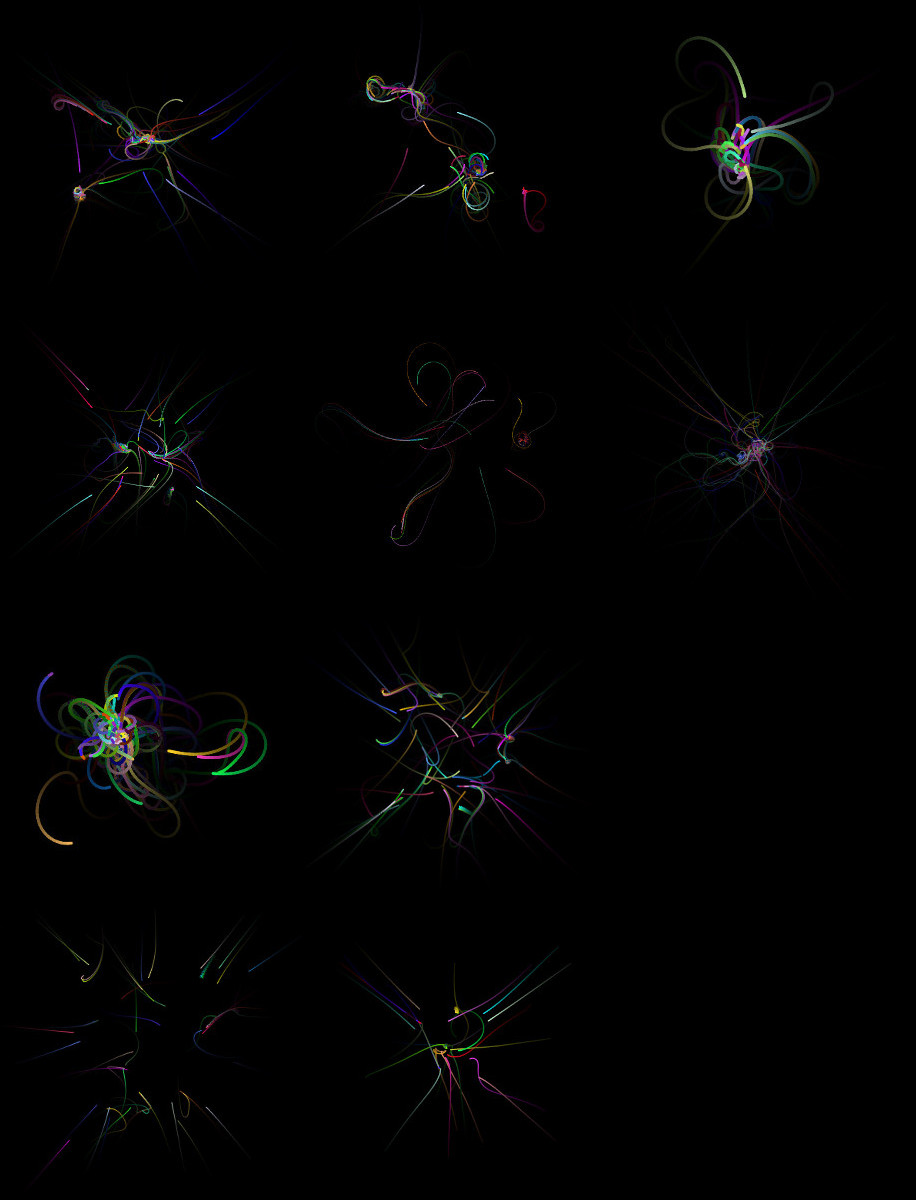
\includegraphics[width=10cm]{./fireflower.jpg}\\
\end{figure}
\end{center}
\begin{center}
\begin{figure}[H]
\centering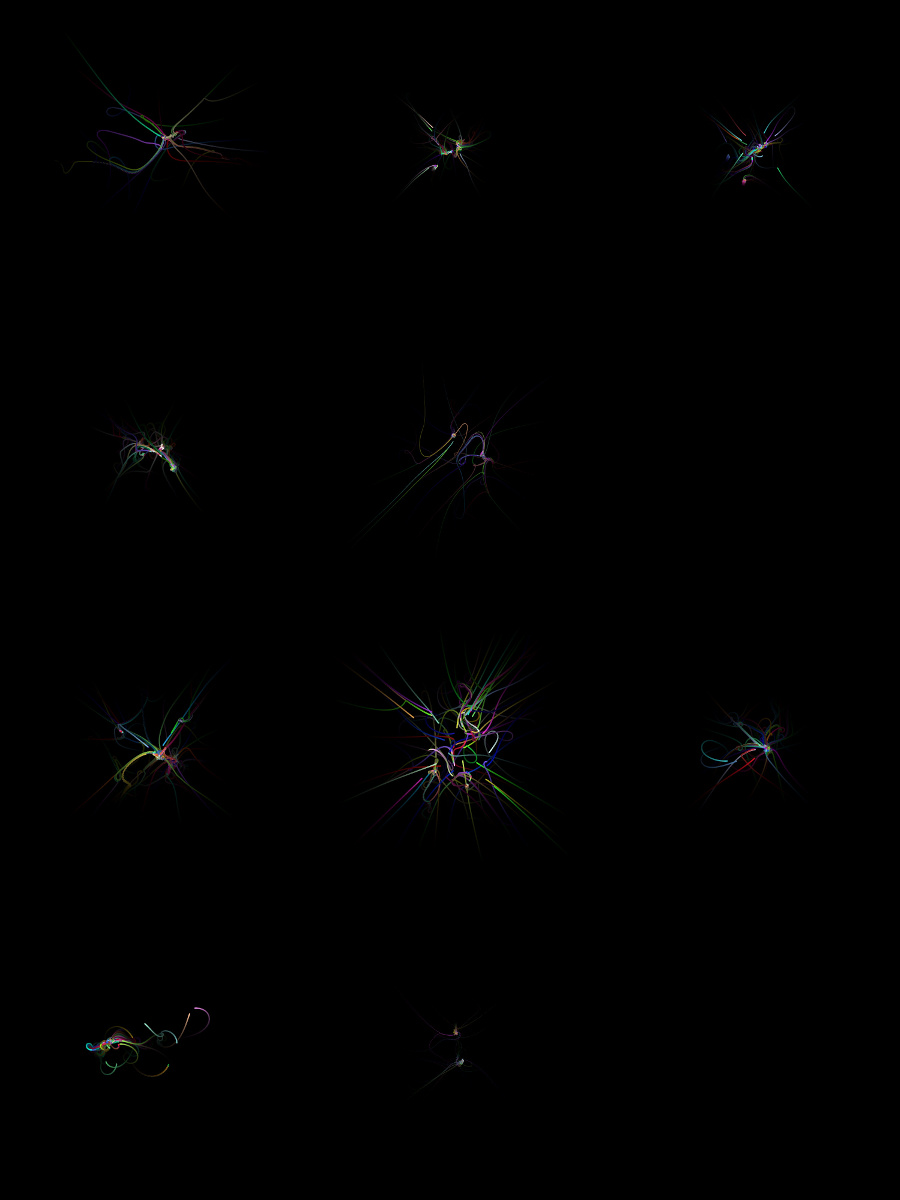
\includegraphics[width=10cm]{./fireflower2.jpg}\\
\end{figure}
\end{center}

\end{document}


